\section{The \protect\Erdos\ Unit Distance Problem}

The \Erdos\ Unit Distance Problem asks the following question:
\begin{center}
    \textbf{How many unit distances can there be amongst $n$ distinct points in $\R^2$?}
\end{center}

\subsection{Lower Bounds}

Some naïve constructions include making each point adjacent to four or six others by way of square/triangular tiling.
\begin{figure}[H]
    \centering
    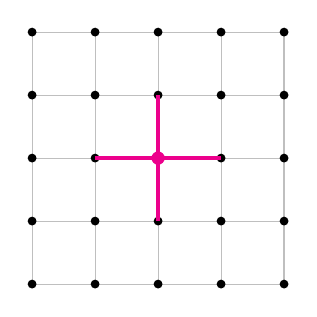
\begin{tikzpicture}[scale = 0.8]
        \draw[gray!50] (-2, -2) grid (2, 2);
        \foreach \x in {-2, ..., 2}{
            \foreach \y in {-2, ..., 2}{
                \fill[black] (\x, \y) circle (2pt);
            }
        }
        \foreach \ang in {0, 90, 180, 270}{
            \draw[very thick, magenta] (0, 0) -- (\ang:1);
        }
        \fill[magenta] (0, 0) circle (3pt);
    \end{tikzpicture}
    \qquad \qquad
    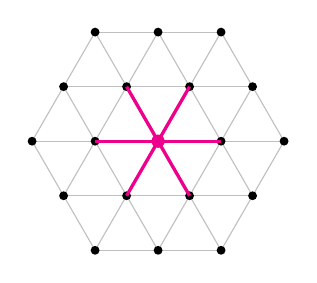
\begin{tikzpicture}[scale = 0.8]
        \foreach \j in {-2, ..., 2}{
            \foreach \i in {-2, ..., 2}{
                \pgfmathtruncatemacro{\hexdist}{max(abs(\i), abs(\j), abs(\i + \j))}
                \ifnum \hexdist < 3
                    \pgfmathsetmacro{\x}{\i + 0.5 * \j}
                    \pgfmathsetmacro{\y}{0.866 * \j}
                    \foreach \di/\dj/\ang in {1/0/0, 0/1/60, -1/1/120}{
                        \pgfmathtruncatemacro{\nextdist}{max(abs(\i + \di), abs(\j + \dj), abs(\i + \di + \j + \dj))}
                        \ifnum \nextdist < 3
                            \draw[gray!50, shift = {(\x, \y)}] (0, 0) -- (\ang:1);
                        \fi
                    }
                    \fill[black] (\x, \y) circle (2pt);
                \fi
            }
        }
        \foreach \ang in {0, 60, ..., 300}{
            \draw[very thick, magenta] (0, 0) -- (\ang:1);
        }
        \fill[magenta] (0, 0) circle (3pt);
    \end{tikzpicture}
\end{figure}

Another construction gives us even better numbers.

Take a square. Each vertex is connected to $2$ others. Translate it by one unit and connect it. Then each vertex is connected to $3$ others. Translate it by another unit and connect it again. Then each vertex is connected to $4$ others. Keep going. In this construction, you get $n \log(n)$ as your lower-bound.

More precisely, each translation is by a unit vector in a new direction, and the directions are chosen generically enough (a random choice works) that no two points ever coincide. The square is a $2$-dimensional cube, and each translation adds a dimension, so after $d - 2$ translations we have $n = 2^d$ points, each at unit distance from $d$ others. Each unit distance is counted from both of its ends, so there are at least
\begin{align*}
    \frac{nd}{2} = \frac{1}{2} n \log_2(n)
\end{align*}
of them.

\Erdos\ gave something even better: draw a grid with the points some distance $\frac{1}{R}$ apart, where $R$ has the property that $R^2 = a^2 + b^2$ in many ways. The point is that this looks like the following:
\begin{figure}[H]
    \centering
    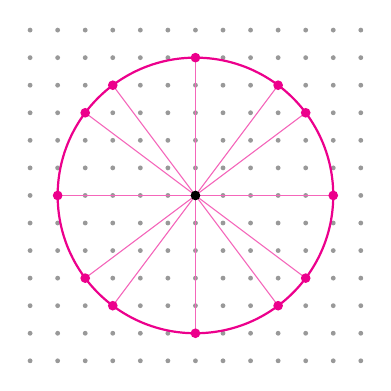
\begin{tikzpicture}[scale = 0.35]
        \foreach \x in {-6, ..., 6}{
            \foreach \y in {-6, ..., 6}{
                \fill[black!40] (\x, \y) circle (2.5pt);
            }
        }
        \draw[thick, magenta] (0, 0) circle (5);
        \foreach \x/\y in {5/0, 4/3, 3/4, 0/5, -3/4, -4/3, -5/0, -4/-3, -3/-4, 0/-5, 3/-4, 4/-3}{
            \draw[magenta!60] (0, 0) -- (\x, \y);
            \fill[magenta] (\x, \y) circle (5pt);
        }
        \fill[black] (0, 0) circle (5pt);
    \end{tikzpicture}
\end{figure}
Here $R = 5$, and $25 = 0^2 + 5^2 = 3^2 + 4^2 = 4^2 + 3^2$ puts $12$ grid points on the circle of radius $R$ grid units, ie, at unit distance from the centre.

We can then do some very nice algebraic number theory involving $\Z[i]$ to get
\begin{align*}
    n^{1 + \frac{c}{\log\of{\log(n)}}}
\end{align*}

\Erdos\ conjectured that the maximum you could get to is $n^{1 + o(1)}$. OpenAI disproved this by finding an $n^{1 + \delta}$ construction for some $\delta > 0$.

% [CORRECTED] was: "an upper-bound: $n^{\frac{4}{3}}$" --- the Spencer--Szemer\'{e}di--Trotter bound has a constant
% in it, and the best known one is above $1$; with constant $1$ it is not a theorem.
We will not get into the lower-bounds here, but we will show an upper-bound: $\BigO{n^{\frac{4}{3}}}$. The tool for it is drawing graphs in the plane.

\subsection{Planar Graphs}

We also make a distinction between plane and planar graphs: planar graphs are abstract graphs with drawings in the plane, and plane graphs are the actual drawings themselves. More formally, we define the following.

\begin{boxdefinition}[Planar Graph]
    A graph $G$ is \textbf{planar} if it has an \textbf{embedding} in the plane: an injective map sending each vertex to a point of $\R^2$ and each edge $\set{u, v}$ to a curve joining the images of $u$ and $v$, such that no curve passes through the image of any other vertex and no two curves meet except at a common endpoint.
\end{boxdefinition}

The picture itself is then the following.

\begin{boxdefinition}[Plane Graph]
    A \textbf{plane graph} is the image of an embedding of a planar graph: the points and curves in $\R^2$ themselves. Its \textbf{faces} are the connected components of what remains of $\R^2$ once the plane graph is removed.
\end{boxdefinition}

Not all graphs are planar.

\begin{boxnexample}[Non-planar graphs]
    $K_5$, $K_{100}$, any $K_n$ for $n \geq 5$.
    \begin{figure}[H]
        \centering
        \begin{tikzpicture}
            \completegraph{5}
        \end{tikzpicture}
    \end{figure}
\end{boxnexample}

The reason graphs fail to be planar is that too many of their edges cross.

We follow the lecture's letters for the sizes of a graph.

\begin{boxlnotation}
    For the rest of this section, a graph $G$ has $n$ vertices and $m$ edges, and a plane graph has $f$ faces. Where several graphs are in play, we write $n(H)$ and $m(H)$ for the numbers of vertices and edges of $H$.
\end{boxlnotation}

(Connected) plane graphs satisfy Euler's Formula: $n - m + f = 2$. We can prove this using induction on $m$ and some handwaving (one should say ``visual intuition''), but to actually do this rigorously takes a lot of machinery (eg. the Jordan Curve Theorem).

\begin{boxtheorem}[Euler's Formula]
    For a connected plane graph with $n$ vertices, $m$ edges and $f$ faces,
    \begin{align*}
        n - m + f = 2
    \end{align*}
\end{boxtheorem}
\begin{proof}
    Induction on $m$. \sorry % [CLAUDE] don't fill this in, it's an exercise for me to do later.
\end{proof}

% [CORRECTED] was: "in any plane graph" --- a single edge, or a path with two edges, is a plane graph with one face
% incident with fewer than $3$ edges, and a loop or a pair of parallel edges bounds such a face too. The
% proposition below, which is what uses the first item, assumes this (and connectedness besides).
Notice that in any simple plane graph with at least $3$ edges, we \textit{must} have
\begin{itemize}
    \item Every face is incident with $\geq 3$ edges
    \item Every edge is incident with $\leq 2$ faces
\end{itemize}

This gives us an important inequality.

\begin{boxproposition} \label{Ch7:Prop:Planar_Edge_Bound}
    For any connected simple plane graph with $n$ vertices, $m$ edges and $f$ faces, if $m \geq 3$, then
    \begin{align*}
        m \leq 3n - 6
    \end{align*}
\end{boxproposition}
\begin{proof}
    Count edge-face incidences. By above,
    \begin{align*}
        3f \leq \sum_{F \text{ a face}} \#\!\set{\text{edges $F$ is incident with}} = \sum_{E \text{ an edge}} \#\!\set{\text{faces $E$ is incident with}} \leq 2m
    \end{align*}
    Thus, we get the equivalent inequalities
    \begin{align*}
        3f \leq 2m \qquad \iff  \qquad f \leq \frac{2m}{3}
    \end{align*}
    Combining with Euler's formula, we get
    \begin{align*}
        2
        = n - m + f
        \leq n - m + \frac{2m}{3}
        = n - \frac{m}{3}
    \end{align*}
    Rearranging gives us the desired inequality.
\end{proof}

\subsection{Crossing Numbers}

A graph that is not planar can still be drawn in the plane, and we can ask how few crossings it needs.

\begin{boxdefinition}[Crossing Number]
    For every finite simple graph $G$, define the \textbf{crossing number}, denoted $\pcr{G}$, to be the minimum number of crossings between edges, taken over all drawings of $G$ in the plane. Ie, define
    \begin{align*}
        \pcr{G} = \min_{\text{drawings of $G$ in the plane}} \#\!\set{\text{crossings between edges}}
    \end{align*}
\end{boxdefinition}

We might expect $\pcr{K_n} = \BigO{\parenth{\#\text{edges}}^2} = \BigO{n^4}$.

\Cref{Ch7:Prop:Planar_Edge_Bound} gives us a first lower bound.

\begin{boxlemma} \label{Ch7:Lemma:Crossing_Edge_Bound}
    If $G$ is simple, then $\pcr{G} \geq m - 3n$.
\end{boxlemma}
% [FILLED] proof supplied here; the lecture stated the lemma without proving it
\begin{proof}
    First, every simple plane graph $H$ has $m(H) \leq 3n(H)$. Indeed, each connected component of $H$ is a connected simple plane graph in its own right: a component with $n_i$ vertices and $m_i \geq 3$ edges has $m_i \leq 3n_i - 6 \leq 3n_i$ by \Cref{Ch7:Prop:Planar_Edge_Bound}, and one with $m_i \leq 2$ edges has $m_i \leq 3n_i$ since $n_i \geq 1$. Summing over the components gives $m(H) \leq 3n(H)$.

    Now take a drawing of $G$ with exactly $\pcr{G}$ crossings, and for each crossing delete one of the two edges involved. We have deleted at most $\pcr{G}$ edges, and what remains is a drawing with no crossings at all, ie, a simple plane graph on the same $n$ vertices with at least $m - \pcr{G}$ edges. Thus $m - \pcr{G} \leq 3n$, which rearranges to $\pcr{G} \geq m - 3n$.
\end{proof}

Consider the case $G = K_n$. So $m = \binom{n}{2}$. The above inequality gives us
\begin{align*}
    \pcr{K_n} \geq \binom{n}{2} - 3n
\end{align*}
But we can probably do better than this: we'd at least expect each edge to cross each other edge or something, so we might think $\pcr{K_n} = \Omega\of{n^4}$.

\subsection{The Crossing Lemma}

Probabilistic methods to the rescue!

\begin{boxlnotation}
    Given a graph $G$ and $p \in [0, 1]$, define $G_p$ to be the graph that retains vertices of $G$ independently with probability $p$ (ie, that deletes vertices of $G$ independently with probability $1 - p$). Define random variables $n_p$ and $m_p$, respectively denoting the number of vertices and edges in $G_p$. Denote by $n$ and $m$ the number of vertices and edges respectively of $G$.
\end{boxlnotation}

We actually want to think of $G_p$ as the space of all subgraphs of $G$, with the power sigma algebra, with each singleton (ie, the probability of each subgraph being realised) having probability determined by $p$.

\begin{boxlemma} \label{Ch7:Lemma:Gp_Expectations}
    $\E\of{n_p} = p \cdot n$ and $\E\of{m_p} = p^2 \cdot m$.
\end{boxlemma}
\begin{proof}[Proof sketch]
    $\E\of{n_p} = p \cdot n$ is clear. To compute $\E\of{m_p}$, define indicator random variables $\xi_e$ for each edge $e$, so that $m_p$ is the sum over all edges $e$ of the $\xi_e$. Then apply linearity of expectation.
\end{proof}

We can relate $\pcr{G_p}$ with $\pcr{G}$.

\begin{boxlemma} \label{Ch7:Lemma:Gp_Crossings}
    $\E\of{\pcr{G_p}} \leq p^4 \cdot \pcr{G}$
\end{boxlemma}
\begin{proof}
    \sorry
    % Hint: fix a drawing of $G$ with exactly $\pcr{G}$ crossings, and draw each outcome of $G_p$ by erasing the deleted vertices and every edge at them. This is a drawing of $G_p$, so $\pcr{G_p}$ is at most the number of crossings that survive into it. When does a crossing survive, and with what probability? Then take expectations.
    % Second hint, for the probability: you want the two edges at a crossing to have four distinct endpoints between them. In a drawing with the fewest crossings, two edges that share an endpoint never cross --- if they did, swapping their two pieces between the shared endpoint and the crossing point, and pulling them slightly apart, would give a drawing with fewer crossings.
\end{proof}

If we can then find a tighter lower-bound for $\pcr{G_p}$, we can get a tighter lower-bound for $\pcr{G}$. If we then optimise it by finding the $p$ that makes it tightest, we can actually do a bit better than what we've done so far.

This is the content of the following theorem.

% [FILLED] statement and proof written up from the blackboard photographs supplied with the post-lecture pass of 2026-10-27; the \sorry in the proof is left as an exercise, with a hint
\begin{boxtheorem}[The Crossing Lemma] \label{Ch7:Thm:Crossing_Lemma}
    If $G$ is a simple graph with $n$ vertices and $m \geq 4n$ edges, then
    \begin{align*}
        \pcr{G} \geq \frac{m^3}{64n^2}
    \end{align*}
\end{boxtheorem}
\begin{proof}
    We claim that for every $p \in (0, 1]$,
    \begin{align*}
        p^4 \pcr{G} \geq p^2 m - 3pn
    \end{align*}
    \sorry
    % Hint: every outcome of $G_p$ is a simple graph, so \Cref{Ch7:Lemma:Crossing_Edge_Bound} applies to it. That gives an inequality between three random variables; take expectations of both sides, and bring in \Cref{Ch7:Lemma:Gp_Expectations,Ch7:Lemma:Gp_Crossings}.

    Dividing through by $p^4$, we get
    \begin{align*}
        \pcr{G} \geq \frac{m}{p^2} - \frac{3n}{p^3}
    \end{align*}
    for every $p \in (0, 1]$, and we are free to choose $p$. We take $p = \frac{4n}{m}$, which is a probability precisely because $m \geq 4n$. (This is not quite the $p$ that maximises the right-hand side, but it makes the constant come out cleanly.) Substituting,
    \begin{align*}
        \pcr{G}
        \geq \frac{m^3}{16n^2} - \frac{3m^3}{64n^2}
        = \frac{m^3}{64n^2}
    \end{align*}
\end{proof}

In particular, once $n \geq 9$ we have $\binom{n}{2} \geq 4n$, so
\begin{align*}
    \pcr{K_n}
    \geq \frac{1}{64n^2} \binom{n}{2}^3
    = \frac{n\parenth{n - 1}^3}{512}
    = \Omega\of{n^4}
\end{align*}

\subsection{A Unit-Distance Upper-Bound}

% Written up from the blackboard photographs supplied with the post-lecture pass of 2026-10-27; the three parts of the lemma are left \sorry as exercises, with hints
We can now give the upper-bound we promised. Throughout this subsection, fix a set $X$ of $n$ points in $\R^2$, with $m$ unit distances among them. For each $p \in X$, let $C_p$ be the unit circle centred at $p$, and let $\deg(p)$ be the number of points of $X$ on $C_p$: its degree in the unit distance graph on $X$. Each unit distance is counted at both of its ends, so
\begin{align*}
    2m = \sum_{p \in X} \deg(p)
\end{align*}

The idea is to draw a graph on $X$ using these circles, and to play the crossing lemma off against the fact that circles cannot cross each other very often. Discard every circle $C_p$ with $\deg(p) \leq 2$. Each remaining circle passes through at least $3$ points of $X$, which cut it into $\deg(p)$ arcs. Let $D$ be the drawing whose vertices are the points of $X$ and whose edges are all of these arcs, from all of the remaining circles.
\begin{figure}[H]
    \centering
    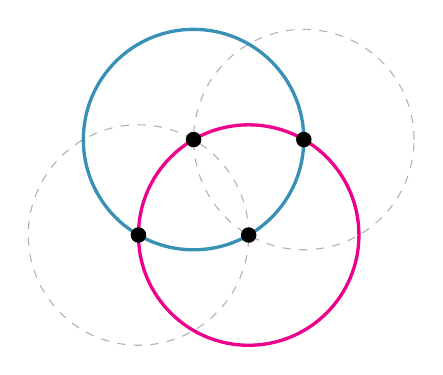
\begin{tikzpicture}[scale = 1.4]
        \draw[gray!60, dashed] (0, 0) circle (1);
        \draw[gray!60, dashed] (1.5, 0.866) circle (1);
        \draw[very thick, magenta] (1, 0) circle (1);
        \draw[very thick, cyan!70!black] (0.5, 0.866) circle (1);
        \foreach \x/\y in {0/0, 1/0, 0.5/0.866, 1.5/0.866}{
            \fill[black] (\x, \y) circle (2pt);
        }
    \end{tikzpicture}
\end{figure}
Here $n = 4$ and $m = 5$. The two dashed circles pass through only two points each and are discarded; each solid circle is cut into three arcs, so $D$ has $6$ edges, and the two long arcs both join the bottom-left point to the top-right one.

That last observation is the catch: two points can be joined by more than one arc, so $D$ is a drawing of a multigraph rather than a graph. But not by much.

\begin{boxlemma} \label{Ch7:Lemma:Circle_Drawing} \hfill
    \begin{enumerate}[label = (\arabic*)]
        \item $D$ has at least $2m - 2n$ edges.
        \item No two vertices of $D$ are joined by more than $2$ edges.
        \item There are at most $n^2$ crossings between edges of $D$.
    \end{enumerate}
\end{boxlemma}
\begin{proof} \hfill
    \begin{description}
        \item[\underline{(1).}] \sorry
        % Hint: how many edges does each remaining circle contribute? Compare the total with $2m = \sum_p \deg(p)$: how much can discarding the circles with $\deg(p) \leq 2$ have cost?
        \item[\underline{(2).}] \sorry
        % Hint: if an arc of $C_p$ joins $u$ and $v$, then $p$ is at distance $1$ from both of them. How many such points $p$ are there? And how many of the arcs of a single circle through at least $3$ points can join $u$ to $v$?
        \item[\underline{(3).}] \sorry
        % Hint: two arcs of the same circle never cross. Two different circles meet in at most $2$ points, and at each of these at most one arc of each circle passes through. Now count pairs of circles.
    \end{description}
\end{proof}

Now we just have to throw away the duplicate edges and apply the crossing lemma.

\begin{boxtheorem} \label{Ch7:Thm:Unit_Distance_Upper_Bound}
    Among any $n$ points in $\R^2$, there are at most $5n^{\frac{4}{3}}$ unit distances.
\end{boxtheorem}
\begin{proof}
    Let $\overline{D}$ be what remains of $D$ when we keep just one edge between each pair of vertices that $D$ joins. By \Cref{Ch7:Lemma:Circle_Drawing} (2) and then (1), $\overline{D}$ has at least half as many edges as $D$, so at least $m - n$ of them. It is a drawing of a simple graph $\overline{G}$ on $n$ vertices, and its crossings are among those of $D$, so by \Cref{Ch7:Lemma:Circle_Drawing} (3),
    \begin{align*}
        \pcr{\overline{G}} \leq n^2
    \end{align*}
    If $m - n < 4n$, then $m < 5n \leq 5n^{\frac{4}{3}}$ and we are done. Otherwise $\overline{G}$ has at least $m - n \geq 4n$ edges, and \Cref{Ch7:Thm:Crossing_Lemma} gives
    \begin{align*}
        n^2 \geq \pcr{\overline{G}} \geq \frac{\parenth{m - n}^3}{64n^2}
    \end{align*}
    Thus $\parenth{m - n}^3 \leq 64n^4$, ie, $m - n \leq 4n^{\frac{4}{3}}$, and $m \leq 4n^{\frac{4}{3}} + n \leq 5n^{\frac{4}{3}}$.
\end{proof}
